%!TEX root = francis_thesis.tex
%%%%%%%%%%%%%%%%%%%%%%%%%%%%%%%%%%%%%%%%%%%%%%%%%%%%%%%%%%%%%%%%%%%%%%%
\chapter{Chapter about theory}\label{ch:THEORY}
\section{Computer Vision Tasks}
With the advance of computer vision, task in computer vision has moved from simple tasks  of image classifaication to complex task like semantic and instance segmentation. 
\subsection{Image Classification}
Image classification investigates the numerical properties of the different picture includes and sorts out information into classifications. Grouping calculations commonly utilize two periods of preparing: preparing and testing. In the underlying preparing stage, trademark properties of common picture highlights are confined and, in light of these, a one of a kind depiction of every grouping class, for example, instructional course, is made. In the resulting testing stage, these component space parcels are utilized to group picture highlights. The depiction of instructional courses is a critical part of the characterization procedure. In the regulated arrangement, factual procedures (for example in light of a from the earlier learning of likelihood conveyance capacities) or dissemination free procedures can be utilized to concentrate class descriptors. The unsupervised classification depends on bunching calculations to naturally section the preparation information into model classes. In either case, the propelling criteria for building instructional courses are that they are:
\begin{enumerate}
\item Independent, e.a change in the description of one training class should not change the value of another,
\item Discriminatory, e.different image features should have significantly different descriptions, and
\item Reliable, all image features within a training group should share the common definitive descriptions of that group.
\end{enumerate}

 This representation allows us to consider each image feature as occupying a point, and each training class as occupying a sub-space (i.e. a representative point surrounded by some spread, or deviation), within the n-dimensional classification space. Viewed as such, the classification problem is that of determining to which sub-space class each feature vector belongs.
\begin{figure}[H]
  \centering
  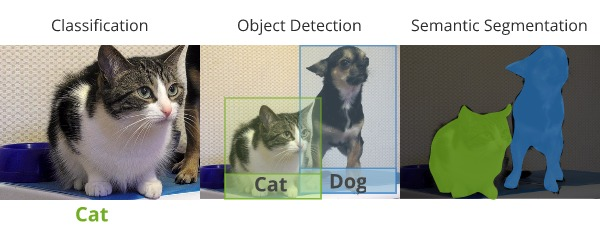
\includegraphics[height=2in]{images/classification_detection_segmentaion_comparisons.jpeg}
   \caption{Image Classification,Object detection Semantic Segmentation.}
\end{figure}
\subsection{Object Detection}
 The objective of object detection is to identify all cases of objects from a referred to class, for example, individuals, vehicles or faces in a picture. Normally just a few occurrences of the item are available in the picture, yet there is an enormous number of potential areas and scales at which they can happen and that need to by one way or another be investigated. 
 Every location is accounted for with some type of posture data. This could be as straightforward as the area of the item, an area, and scale, or the degree of the article characterized as far as a jumping box. In different circumstances, the posture data is progressively nitty gritty and contains the parameters of a straight or non-direct change. For instance, a face identifier may process the areas of the 
 eyes, nose, and mouth, notwithstanding the jumping box of the face. A case of a vehicle and individual discovery that determines the areas of specific parts appears in Figure 1. The posture could likewise be characterized by a three-dimensional change determining the area of the article with respect to the camera. 
 Item discovery frameworks develop a model for an article class from a lot of 
 preparing precedents. On account of a fixed inflexible article, just a single precedent might be 
 required, however more by and large numerous preparation precedents are important to catch 
 
 certain parts of class changeability.
\begin{figure}[H]
  \centering
  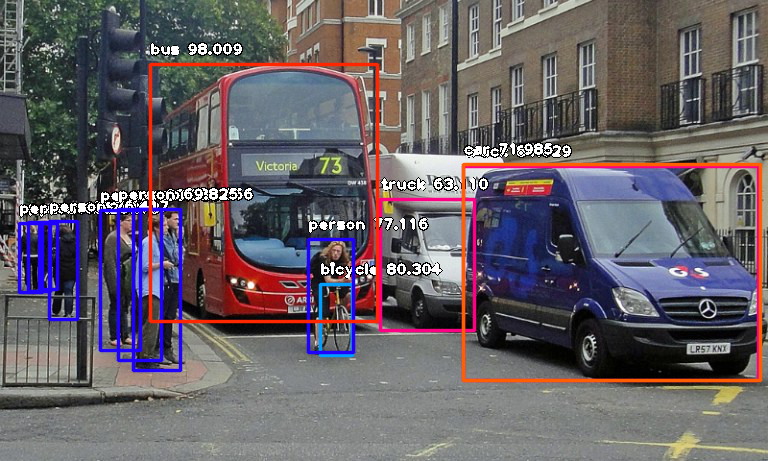
\includegraphics[height=3in]{images/object_det.jpeg}
   \caption{Object detection with bounding boxes.}
\end{figure}

Object detection strategies fall into two noteworthy classes, generative and discriminative. The principal comprises of a likelihood model for the posture changeability of the articles together with an appearance model: a likelihood model for the picture appearance restrictive on a given posture, together with a model for foundation, for example, non-object pictures. The model parameters can be assessed from preparing information and the choices depend on proportions of back probabilities. The second regularly manufactures a classifier that can segregate between pictures (or sub-images) containing the item and those not containing the object. The parameters of the classifier are chosen to limit botches on the training data, frequently with a regularization bias to abstain from overfitting. Different qualifications among discovery calculations have to do with the computational apparatuses used to check the whole picture or search over potential represents, the sort of picture portrayal with which the models are developed, and what type and how much training data is required to construct a model.


\subsection{
Semantic Segmentation
}
Segmentation is fundamental for picture analysis assignments. Semantic segmentation portrays the way toward partner every pixel of a picture with a class name, (for example, bloom, individual, street, sky, sea, or vehicle). 

Semantic image segmentation can be connected successfully to any errand that includes the division of visual data. Precedents incorporate street division for self-ruling vehicles, restorative picture division, scene division for robot observation, and in picture altering apparatuses. While at present accessible frameworks give precise article acknowledgment, they are unfit to depict the limits between items with a similar exactness. 

Oxford scientists have built up a novel neural system segment for a semantic division that improves the capacity to perceive and depict objects. This development can be connected to improve any circumstance requiring the division of visual data. 

Semantic image segmentation assumes a vital job in picture understanding, enabling a computer to perceive questions in pictures. Acknowledgment and depiction of articles are accomplished through the order of every pixel in a picture. Such procedures have a wide scope of utilization in PC vision, in differing and developing fields, for example, vehicle self-sufficiency and restorative imaging. 

The past best in class picture division frameworks utilized Fully Convolutional Neural Network (FCNN) segments, which offer magnificent exactness in perceiving objects. While this advancement spoke to a huge improvement in the semantic division, these systems don't perform well in depicting object limits. Conditional Random Fields  (CRFs) can be utilized in a post-handling venture to improve object limit depiction, be that as it may, this isn't an ideal arrangement inferable from an absence of reconciliation with the profound system.
\begin{figure}[H]
  \centering
  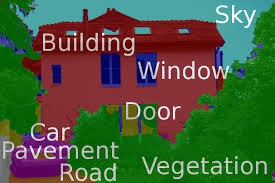
\includegraphics[height=3in]{images/semantic.jpg}
   \caption{Image with semantic segmentation.}
\end{figure}
Oxford specialists have built up a neural system segment for semantic segmentation that bridles the outstanding article acknowledgment of FCNNs and the incredible limit depiction of CRFs. CRFs are completely incorporated as repetitive neural systems, bringing about a framework that offers upgraded execution contrasted with the past cutting edge. The tale framework can be connected to any assignment that includes the division of visual data. Precedents incorporate street division for independent vehicles, restorative picture division, scene division for robot recognition, and in picture altering instruments. Oxford University Innovation is looking for modern accomplices that desire to investigate the utilization of this framework for business applications.
\subsection{
Instance Segmentation
}
Instance segmentation is one stage in front of semantic division wherein alongside pixel level grouping, we anticipate that the computer should characterize each occurrence of a class independently. For instance in the picture above there are 3 individuals, actually 3 examples of the class "Person". All the 3 are characterized independently (in an alternate shading). Yet, the semantic division does not separate between the examples of a specific class.
\begin{figure}[H]
  \centering
  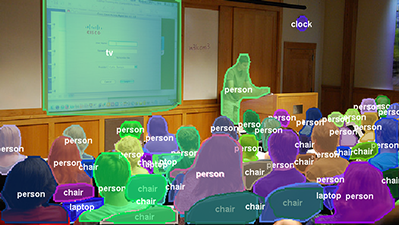
\includegraphics[height=3in]{images/instance.png}
   \caption{Image with instance segmentation.}
\end{figure}

\section{CNN for Object Detection and  Segmentation }
Mask RCNN is a profound neural system meant to take care of occurrence division issue in machine learning or computer vision. As it were, it can isolate various items in a picture or a video. You give it a picture, it gives you the object bouncing boxes, classes and masks. 

There are two phases of Mask RCNN. Initially, it produces proposals about the areas where there may be an object dependent on the input picture. Second, it predicts the class of the object, refines the bounding box and produces a masks in pixel dimension of the item dependent on the primary stage proposition. The two phases are associated with the backbone structure. We will describe Mask R-CNN fully below. We have four components of Mask R-CNN viz; The backbone, Regional Proposal Network,{ROI Classifier and Bounding Box Regressor,Segmentation mask. These components will be discussed in detail in the sections below.
\subsection{Backbone}
\subsubsection{Residual Networks (RESNET)}
ResNet is an essential neural network that serves as a backbone to Mask R-CNN and numerous computer vision tasks. 
It makes the training of extremely deep neural networks possible which was very difficult before then due to the 
challenge of vanishing gradients, that hampers convergence in the network. According to \protect\cite{M} before RESNET, the problem 
of \textit{vanishing gradient} has been mainly addressed by normalized initialization \protect\cite{N},\protect\cite{O}, \protect\cite{P}, \protect\cite{Q} and intermediate 
normalization layers \protect\cite{R}, which enable networks with tens of layers to start converging for stochastic gradient descent 
(SGD) with backpropagation \protect\cite{S}.
Looking at the sample scenario of the vanishing gradients or degradation. A worst-case scenario of vanishing gradient is
 the case was the early layers of a deeper model can be replaced with a shallow network and the other layers can act as an identity function.  The shallow network and its deeper counterpart give the same accuracy. So deeper models do not perform well due to degradation. When a deeper network is used it approximates the mapping than its shallower variant and decreases the error by a notable margin. 
 Also, the deeper network had issues of degradation.
To solve this problem ResNet introduced the concept of skip connection.

\begin{figure}[H]
 \centering
 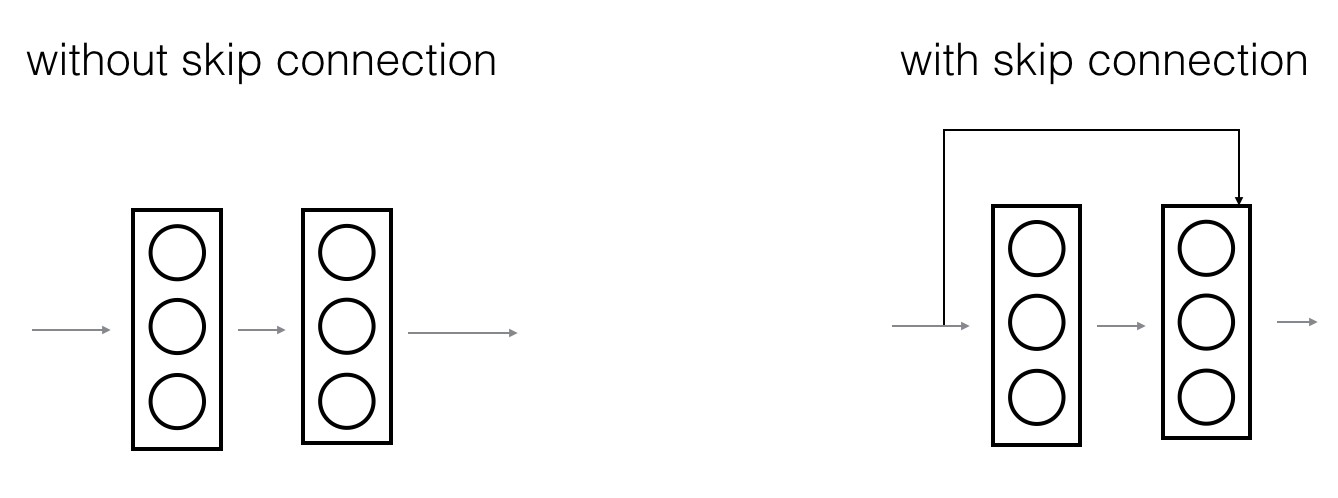
\includegraphics[height=2.3in]{images/skipconnection.jpg}
 \caption{Skip connection of ResNet.}
\end{figure}

Without a skip connection, deep convolution networks are stacked together one after the other.  With a skip connection deep convolution networks are tacked together but this time the original input is added to the output of the convolution block.
Mathematically representing this, we can consider a mapping or space G(x) to be fitted by some stacked layers of an entire network.  X denotes the inputs in the first layer of the net. This layer will approximate a residual function Z(x) = G(x)-x by hypothesizing.  Therefore the original function or mapping G(x) becomes Z(x) + x.  The input and output dimensions are expected to be of the same dimension for this work properly.  It is worth noting that ResNet, contained 152 layers, won ILSVRC 2015 with an error rate of 3.6 percent beating even humans with their error rate of circa 5 – 10 percent, and replacing VGG-16 layers in Faster R-CNN with ResNet-101 produced relative improvements of 28 percent. It also trained networks with 100 layers and 1000 layers. 

\begin{figure}[H]
  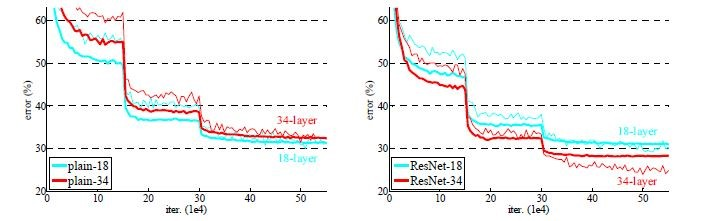
\includegraphics[height=2.2in]{images/resnet-graph.jpg}
   \caption{Training on ImageNet. Thin curves denote training error, and bold curves denote validation error of the center crops. Left: plain networks of 18 and 34 layers. Right: ResNets of 18 and 34 layers. In this plot, the residual networks have no extra parameter compared to their plain counterparts \protect\cite{M}.}
\end{figure}

\subsubsection{Feature Pyramid Network}
Feature Pyramid Network (FPN) is a generic feature extractor used in various application for recognizing objects at different scales, developed by Lin et al [K]. For the recognition system for detecting objects at various scales, feature pyramid is a primary constituent of such a system. Pyramid representation has the problem of computing and memory intensiveness and has been avoided in the deep learning object detectors. 
Feature Pyramid Network (FPN) solves this problem by restructuring the architecture of the pyramid to a top-down architecture with lateral connections. The multi-scale, pyramidal hierarchy of deep ConvNet was leveraged to develop Feature Pyramid Network (FPN). Pyramids of  FPN are scale-invariant. This means that when an object scale changes it is offset by shifting its level in the pyramid.  
 Before the introduction of FPN, some ways were used in the extraction of features from images. Initially, hand-engineered features \cite{U} were used and it makes use of featurized image pyramids. ConvNet is more robust to variance in scale, capable of representing higher-level semantics, and so features from it have quickly replaced engineered features. 
 According to \cite{L} this ConvNets gives multi-scale feature representation in which all levels are semantically strong, including the high-resolution levels.  Featuring each level of an image pyramid comes with the profound limitation of increase in inference time which makes it impractical for real applications. FPN explored the pyramidal shape of a ConvNet’s feature hierarchy to build a feature pyramid that has strong features
  with high-resolution at all scales. 
 This gives a feature pyramid that has profound semantics at all phases and is constructed quickly  from a unit  input image scale 
\begin{figure}[H]
\centering
  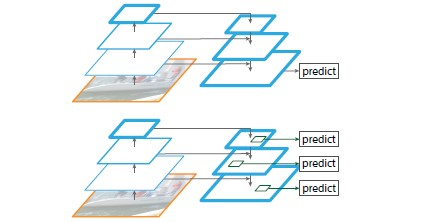
\includegraphics[height=3in]{images/fpn.jpg}
   \caption{Top: a top-down architecture with skip connections, where predictions are made on the finest level (e.g., \protect\cite{T}). Bottom: FPN model that has a similar structure but leverages it as a feature pyramid, with predictions made independently at all levels \protect\cite{K}.}
\end{figure}

FPN was applied in Regional Proposal Network (RPN) and Fast R-CNN. With the new adaptations, RPN could be naturally trained and tested with FPN, Using FPN in a basic Faster R-CNN system, the result surpasses all existing single-model entries including those from the COCO 2016 challenge winners.

\subsection{Regional Proposal Network}
Regional Proposal Network (RPN) is a useful network effectively used in R-CNN that scans the image in a sliding window pattern over the anchors.  It proposes multiple objects that are recognizable in a particular image. The last convolutional layer that is produced by the Faster R-CNN is called the feature map. A proposal is generated for the region where the object lies by sliding over a feature map a network, which is the RPN. RPN suggest where an object lies in an image.
\begin{figure}[H]
\centering
  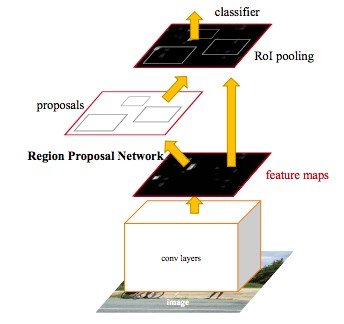
\includegraphics[height=3in]{images/rcnn-rpn.jpg}
   \caption{The architecture of Faster R-CNN. RPN generate the proposal for the objects. \protect\cite{J}.}
\end{figure}

\begin{figure}[H]
\centering
  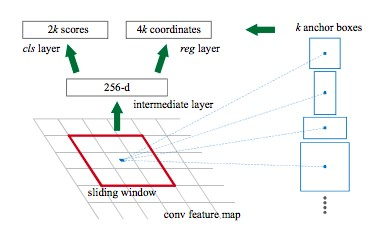
\includegraphics[height=3in]{images/rpn-arch.jpg}
   \caption{RPN Architecture \protect\cite{J}.}
\end{figure}

Analyzing the architecture of RPN, the intermediate layer divides into a classifier and regressor layers, and the 
concept of the anchor was introduced. Anchor are boxes of different sizes and aspect ratio that are generated over an 
image that determines the ideal location, shape, and size of objects in the image. They overlap to fill up as much of 
the image as possible. Thousands of anchor boxes are generated for this. For each anchor box, the object’s bounding box 
that has the highest overlap is divided by non-overlap. This is termed Intersection Over Union (IOU). If the highest IOU 
is greater than 50 percent, the anchor box determines the object that gave the highest IOU. But if it is greater than 40 
percent the true detection is ambiguous, and if it is less than 40 percent it predicts no object. Classifier gives the
 probability of a proposal containing the target object. Regression regresses the coordinates of the proposals. RPN is 
 also used in Mask RCNN.
\begin{figure}[H]
\centering
  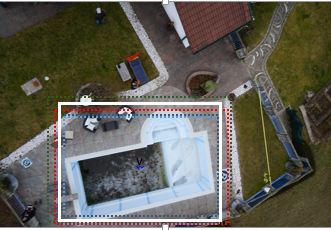
\includegraphics[height=3in]{images/rpn1.png}
   \caption{Anchor boxes (dotted) and the shift/scale applied to them to fit the object precisely (solid). 
   Several anchors can map to the same object.}
\end{figure}

The RPN produces two results for each anchor; Anchor Class i.e. either the foreground or the background, and
 Bounding Box Refinement, an estimation to rectify the anchor box that fits the object well. This is a change in x,y,
  width, height.

\subsection{ROI Classifier and Bounding Box Regressor}
Region of Interest (ROI) classifier is proposed by the Region Proposal Network (RPN) and similarly,
 like the RPN, it produces two results for each ROI. First, the \textit{class}, it produces the classes
  of the object in the ROI, but it is deeper and can classify regions to specific classes (car, person, nucleus, etc). 
  And secondly the\textit{ Bounding Box Refinement}, which further refines the location and size of the bounding box 
  to envelope the object.
\subsubsection{ROI Pooling}
Input sizes of a classifier vary. Classifiers require fixed, stable input size and can’t manage varying input sizes. 
Bounding box refinement in RPN produces ROI boxes of various sizes. ROI Pooling tackles this challenge.
 Cropping a part of a feature map and resizing it to a fixed size is termed ROI pooling. It is very much alike to 
 the concept of resizing a cropped image.
\begin{figure}[H] 
\centering
  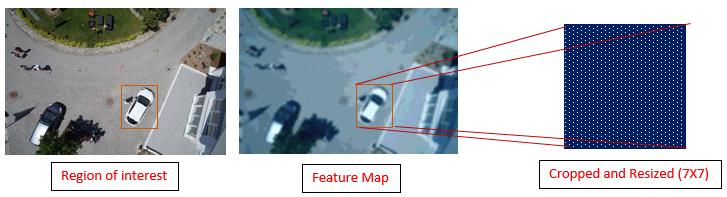
\includegraphics[height=1.8in]{images/roi1.png}
   \caption{ROI Pooling.}
\end{figure}

\subsection{Segmentation Mask}
Mask RCNN further added an extra branch to what Faster RCNN has. This is the mask branch. The Mask branch is a convolutional network that receives the positive regions selected by the ROI classifier and builds low resolution masks for them. The resolution is about 28x 28 pixels. They are soft masks, constituted by float numbers, so they contain more ingredients than binary masks. The size of the mask enables the mask branch to be light. When training the model, the ground-truth masks is scaled down to 28x28 to compute the loss, and when inferencing the predicted masks is scaled up to the size of the ROI bounding box and that produces the final masks, one per object.
\begin{figure}[H]
  \centering
    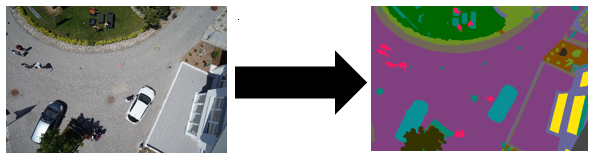
\includegraphics[height=1.7in]{images/mask.png}
     \caption{Segmentation Mask of a drone-based imageset .}
  \end{figure}


\section{Drone-Based Dataset }
Drones (or UAVs) furnished with high resolution cameras have been utilized in a wide range of applications, 
including agricultural, aerial photography, fast delivery, surveillance, etc. This has made, automatic comprehension of 
visual data collected from drones become highly demanding, which brings computer vision to drones more and more closely.
 Outstanding advancements have been made in general computer vision algorithms, such as detection and tracking, yet these algorithms 
 are not usually flawless for dealing with sequences or images captured by drones, due to various difficulties such as view point changes 
 and scales. Consequently, developing and appraising new vision algorithms for drone generated visual data is a key problem in drone-based 
 applications.
The major challenge of segmentation in drone generated visual data is the lack of proper datasets for these. 
A VisDrone Dataset was produced in \protect\cite{V}. The images and video sequences in the benchmark were captured over
 various urban/suburban areas of 14 different cities across China from north to south. Specifically, VisDrone2018 
 consists of 263 video clips and 10; 209 images (no overlap with video clips) with rich annotations, including object 
 bounding boxes, object categories, occlusion, truncation ratios, etc. With intensive amount of effort, our benchmark 
  has more than 2:5 million annotated instances in 179; 264 images/video frames \protect\cite{V}. Also Semantic Drone Dataset that focuses on
   semantic understanding of urban scenes for increasing the safety of autonomous drone flight and landing procedures. The imagery depicts 
   more than 20 houses from nadir (bird's eye) view acquired at an altitude of 5 to 30 meters above ground. A high resolution camera was 
   used to acquire images at a size of 6000x4000px (24Mpx). The training set contains 400 publicly available images and the test set is 
    made up of 200 private images. \protect\cite{W}.

\begin{figure}[H]
  \centering
  
    \includegraphics[height=2.2in]{images/045.jpg}
    \caption{Drone-based imageset 1}
    \label{image 1}
  \end{figure}
  %
  
  \begin{figure}[H]
    \centering
    \includegraphics[height=2.2in]{images/044.jpg}
    \caption{Drone-based imageset 2}
    \label{image 2}
\end{figure}